% !TEX root = ./article.tex

\documentclass{article}

\usepackage{mystyle}
\usepackage{myvars}

%-----------------------------

\begin{document}

	\maketitle
  \thispagestyle{empty}

%-----------------------------
%	TEXT
%-----------------------------

  \section{Demostración de insesgadez}
  \label{sec:demostration_1}

    \paragraph{}
    Para una población población finita $U$ formada por los individuos $\{ 1, ..., i, ..., N\}$ cuya variable de interés se denota por $y$, siendo $y_k$ el valor que toma dicha variable en el individuo $k$. Se define el total poblacional como sigue:
    \begin{align}
      t &= \sum_{k \in U}y_k
    \end{align}

    \paragraph{}
    Sea $s$ una muestra extraida de la población $U$ (por tanto $s \subset U$), se define la variable aleatoria $I_k$ como se indica a continuación:

    \begin{equation}
      I_k =
      \begin{cases}
        1 & \text{si } k \in s \\
        0 & \text{si } k \not\in s
      \end{cases}
    \end{equation}

    \paragraph{}
    De esta manera, se puede utilizar el valor $\pi_k$ para modelizar la probabilidad de que $I_k$ tome el valor $1$, es decir, de que el elemento $k$-ésimo esté en la muestra $s$. Por tanto, se puede afirmar que $I_k \sim B(\pi_k)$, una distribución de \emph{Bernoulli} de parámetro $\pi_k$. A partir de dicha distribución se tiene que $E[I_K] = \pi_k$. Además, $pi_k > 0 \forall k \in U$ para que se cumpla la restricción de muestreo probabilístico.


    \paragraph{}
    Se define el $\pi$-estimador como:

    \begin{equation}
      \widehat{t}_\pi = \sum_{k \in s} \frac{y_k}{\pi_k} = \sum_{k \in U} I_k \frac{y_k}{\pi_k}
    \end{equation}

    \paragraph{}
    La demostración acerca de la insesgadez de este estimador deriva de la esperanza de la variable $I_k$, que toma el valor $\pi_k$, tal y como se indicaba anteriormente, lo cual produce que se anule dicho valor $pi_k$ con el $pi_k$  del divisor del estimador. Además, la restricción de muestreo probabilístico $pi_k > 0 \forall k \in U$ hace que el valor $\widehat{t}_\pi$ exista siempre (no hay división entre 0). Por estas razones se puede decir que el estimador es insesgado. De manera matemática esto se describe a continuación:

    \begin{align}
      E[t] &= \sum_{k \in U} y_k \\
      E[\widehat{t}_\pi] &= \sum_{k \in U} E[I_k] \frac{y_k}{\pi_k} = \sum_{k \in U} \pi_k \frac{y_k}{\pi_k} =\sum_{k \in U} y_k \\
      bias(t, \widehat{t}_\pi) &= \left| E[t] - E[\widehat{t}_\pi] \right| = \left| \sum_{k \in U} y_k - \sum_{k \in U} y_k \right| = 0
    \end{align}

    \paragraph{}
    Nótese por tanto, que el funcionamiento del $\pi$-estimador se basa en la \say{expansión} del conjunto de individuos seleccionados en la muestra $s$, de tal manera que se siga cumpliendo de la forma más precisa posible la distribución de probabilidades de la población $U$.

  \section{Demostración del intervalo de confianza para la varianza}
  \label{sec:demostration_2}

    \paragraph{}
    [TODO ]

    \begin{figure}
      \centering
      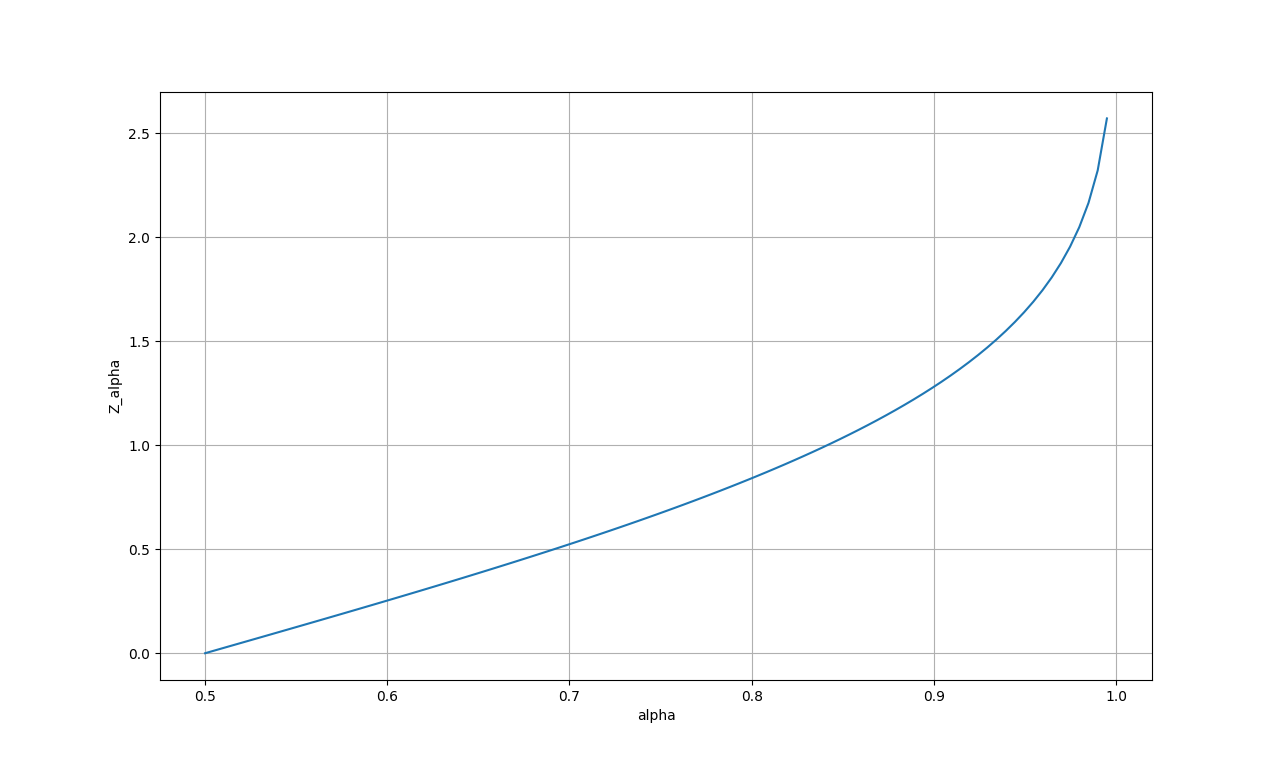
\includegraphics[width=0.75\textwidth]{normal_alpha}
      \caption{}
      \label{}
    \end{figure}

    \begin{align}
      \left[\widehat{t}_\pi \pm z_{1-\alpha/2}\sqrt{\widehat{Var}[\widehat{t}_\pi]}\right]
    \end{align}

    \begin{align}
      \Pr(|X-\widehat{t}_\pi |\leq k \sqrt{Var[\widehat{t}_\pi]} )&\geq {1-\frac {1}{k^{2}}} \\
      \Pr\left(\widehat{t}_\pi - k \sqrt{Var[\widehat{t}_\pi]} \leq X \leq  \widehat{t}_\pi + k \sqrt{Var[\widehat{t}_\pi]} \right)&\geq {1-\frac {1}{k^{2}}} \\
      \Pr\left(X \in \left[\widehat{t}_\pi - k \sqrt{Var[\widehat{t}_\pi]}, \widehat{t}_\pi + k \sqrt{Var[\widehat{t}_\pi]}\right] \right)&\geq {1-\frac {1}{k^{2}}} \\
      \Pr\left(X \in \left[\widehat{t}_\pi \pm k \sqrt{Var[\widehat{t}_\pi]}\right] \right)&\geq {1-\frac {1}{k^{2}}} \\
      \Pr\left(X \in \left[\widehat{t}_\pi \pm z_{1-\alpha/2} \sqrt{Var[\widehat{t}_\pi]}\right] \right)&\geq {1-\frac {1}{z_{1-\alpha/2}^{2}}} \\
      \Pr\left(X \in \left[\widehat{t}_\pi \pm z_{1-\alpha/2} \sqrt{\widehat{Var}[\widehat{t}_\pi]}\right] \right)&\geq {1-\frac {1}{z_{1-\alpha/2}^{2}}}
    \end{align}

%-----------------------------
%	Bibliographic references
%-----------------------------
	\nocite{muest2017}
  \nocite{sarndal2003model}

  \bibliographystyle{alpha}
  \bibliography{bib}

\end{document}
